\documentclass{article}
\author{
	\begin{tabular}{c c}
	&Tom Bednar \\ & Ariella Hanna(Scrum Master) \\ & Alex Honeygosky \\ &Gregg Karanovich
	\end{tabular}
}
\date{September 29, 2016}
\title{CS 1530 - Sprint 1 Deliverable}

\usepackage{indentfirst}
\usepackage{graphicx}
\usepackage{float}

\begin{document}
	\pagenumbering{gobble}
	\maketitle
	\newpage
	\pagenumbering{arabic}
	
	\section{Backlog of User Stories}
	\begin{enumerate}
		\item As a user, I want a chess game that follows the rules of American chess, so that I can
	play the game in the standard way that one would expect.
		\item As a user, I want to be notified when I attempt an illegal move, so that I know it is
	not an error with the program.
		\item As a user, I want a GUI, so that I can see the board and moves on screen.
		\item As a user, I want an indication of whose turn it is, so that I can see when it is my
	turn to go.
		\item As a user, I want black to always be on top and white to always be on bottom because
	that is my preferred way to view the board.
		\item As a user, I want grid coordinates on the outlines, so that I can gain familiarity with
	algebraic notation of chess.
		\item As a user, I want the option to play again, so that I don't have to restart the program
	to start a new game.
		\item As a user, I want a descriptive error message if the program should crash, so that
	I can attempt to avoid that scenario in the future.
		\item As a user, I want to be able to choose between black or white, so that I can choose
	if I want to move first or second.
		\item As a user, I want to make moves by clicking on my piece and then the location, so that
	I can move the pieces in a way that is close to how I would move them in real life.
		\item As a user, I want the AI to take no more than 10 seconds to choose a move because I
	would like to spend more time playing than waiting on the AI.
		\item As a user, I want the option to exit and save the game, so that I can come back to games
	I was unable to finish.
		\item As a user, I want buttons under the board to exit and save the game because that is
	a simple and fast way to save and quit.
		\item As a developer, I want the game to save as a PGN text file because that is the standard.
		\item As a user, I want multiple save and load game states so that I can save more than one
	game at a time.
		\item As a user, I want the option to set a time limit, so that I can play with a time limit.
		\item As a user, I want the option to confirm a move before it's final, so that I can change
	my mind if I make a bad move or undo an accidental click.
		\item As a user, I want taken pieces to show up on the side, so that I can see the pieces I've
	captured and the pieces my opponent has captured.
		\item As a user, I want a tutorial, so that I can learn how to play the game without needing
	an outside source.
		\item As a user, I want the ability to undo my most recent move, so that I can undo accidental
	clicks or go back if I made a bad move.
		\item As a user, I want past moves to display on the side of the board, so that I can see a 
	record of how the game went.
		\item As a user, I want a hint system, so that I can see if the move I was planning is a good
	idea or to get help when I'm stuck.
		\item As a user, I want different difficulty settings, so that I can choose the level of my
	opponent.
	\end{enumerate}
	\newpage
	
	\section{Test and Branching Plan}
	\subsection*{Test Plan}
	One of the biggest aspects of the game which will need testings is whether or not the game follows the correct rules. In this case, chess must follow the rules of American chess. This means all pieces should only be able to make the appropriate moves. If the user attempts an illegal move for a piece, they should be informed and prevented from doing so. Included with the rules is also the ability to take the opponent's pieces. Testing will be necessary to ensure that only the opponents pieces can be taken and not accidentally take your own. These tests are necessary to guarantee that rules of the game are set, followed by the user, and every user is on the same page. \par
	Another aspect needing testing is the GUI itself. All buttons should perform the appropriate functions (i.e. Exit should exit the program, and New Game should start a new game). This also includes the correct placement of the pieces based on the user's mouse click. This specific testing will be required in order to allow the user to reliably play the game without any frustrations. \par
	Though the save function will be a part of the GUI, as it will be a button, it must also be tested separately. The intended goal of saving is to create a PGN which will be stored for later use. Therefore we will need to test whether the correct game state is saved and when loaded, the board is setup correctly. This is key for the user when they wish to continue a game that was started earlier. This feature also adds to the reliability of the game which is key to keep the user coming back. \par
	Other functionalities will need to be tested too. These include undoing a move, producing a hint, and displaying past moves. Undo needs to be tested to ensure the piece is restored to correct position. Displaying past moves must correctly show moves which were performed in the past. Lastly, the hints given must not put the user in a position which results in an immediate check or checkmate. If the hint were to give bad advice, then the user would lose faith in the hints and the game. \par
	\subsection*{Branching Plan}
	\par
	Our branching plan will first consist of individual branches for each member of the team and will be named as such. From there, each new branch will be determined for each major piece of the project. This means we will have branches such as GUI branch, a controller branch, and maybe a model branch. With all this branches we will need to have someone oversee the integration of them. This will be a job for the sprint's Scrum Master. Hopefully this will help prevent any code which could essentially break the program. Note: this branching/integration plan may be changed as the sprints continue.
	\newpage
	
	\section{User Story Methodology}
		The first step in determining our user stories was to listen to what our client said that he wanted and take notes.  We asked questions as well in order to leave little room for interpretation.  The next step was to prioritize these bullet points.  Our client stated things as medium priority, low priority, or with no stated priority. Any bullet point that was not marked low or medium was assumed to be high priority.  We then arranged the bullet points so that they were grouped by priority from high to low.  Then, we went through the list and combined any bullet points that seemed to be saying the same thing.  For example, "follow the rules of American Chess" and "notify the user if they attempt an illegal move and then do not complete the move" could both be under the umbrella of following the rules. \par
		Next, we sorted the bullet points within their groups based on what we felt was most important for a working chess game and then by what we felt would take the least amount of time to complete.  Finally, the last step was to convert these bullet points into user stories.  To do this, we evaluated the bullet points and thought about who wants this feature and why.  For example, looking at the bullet point, "option to play again", we can see that the user would want this option so that they do not have to exit and restart the program to play a new game. 
	\newpage
	\section{Paper Prototype}
	\subsection*{General User Interaction with Laboon Chess}
	The user will first launch the chess game from where ever they have it stored on their computer. Upon launching the game, the user will be presented with the game screen and a pop-up screen that asks them whether they would like to be white or black. Next the user will be taken to the game screen and will be able to play by clicking on their pieces and moving them to valid spaces on the board, per American chess rules. The user will be alerted if they try to make an invalid move. Should the user want to start over, they will be able to press the "New Game" button at the bottom of the screen.  If they would like to save a game or load a previous game, the user will be able to press the "Save Game" or "Load Game" buttons, respectively.
	\begin{figure}[H]
		\caption{Laboon Chess at the start of a game}
		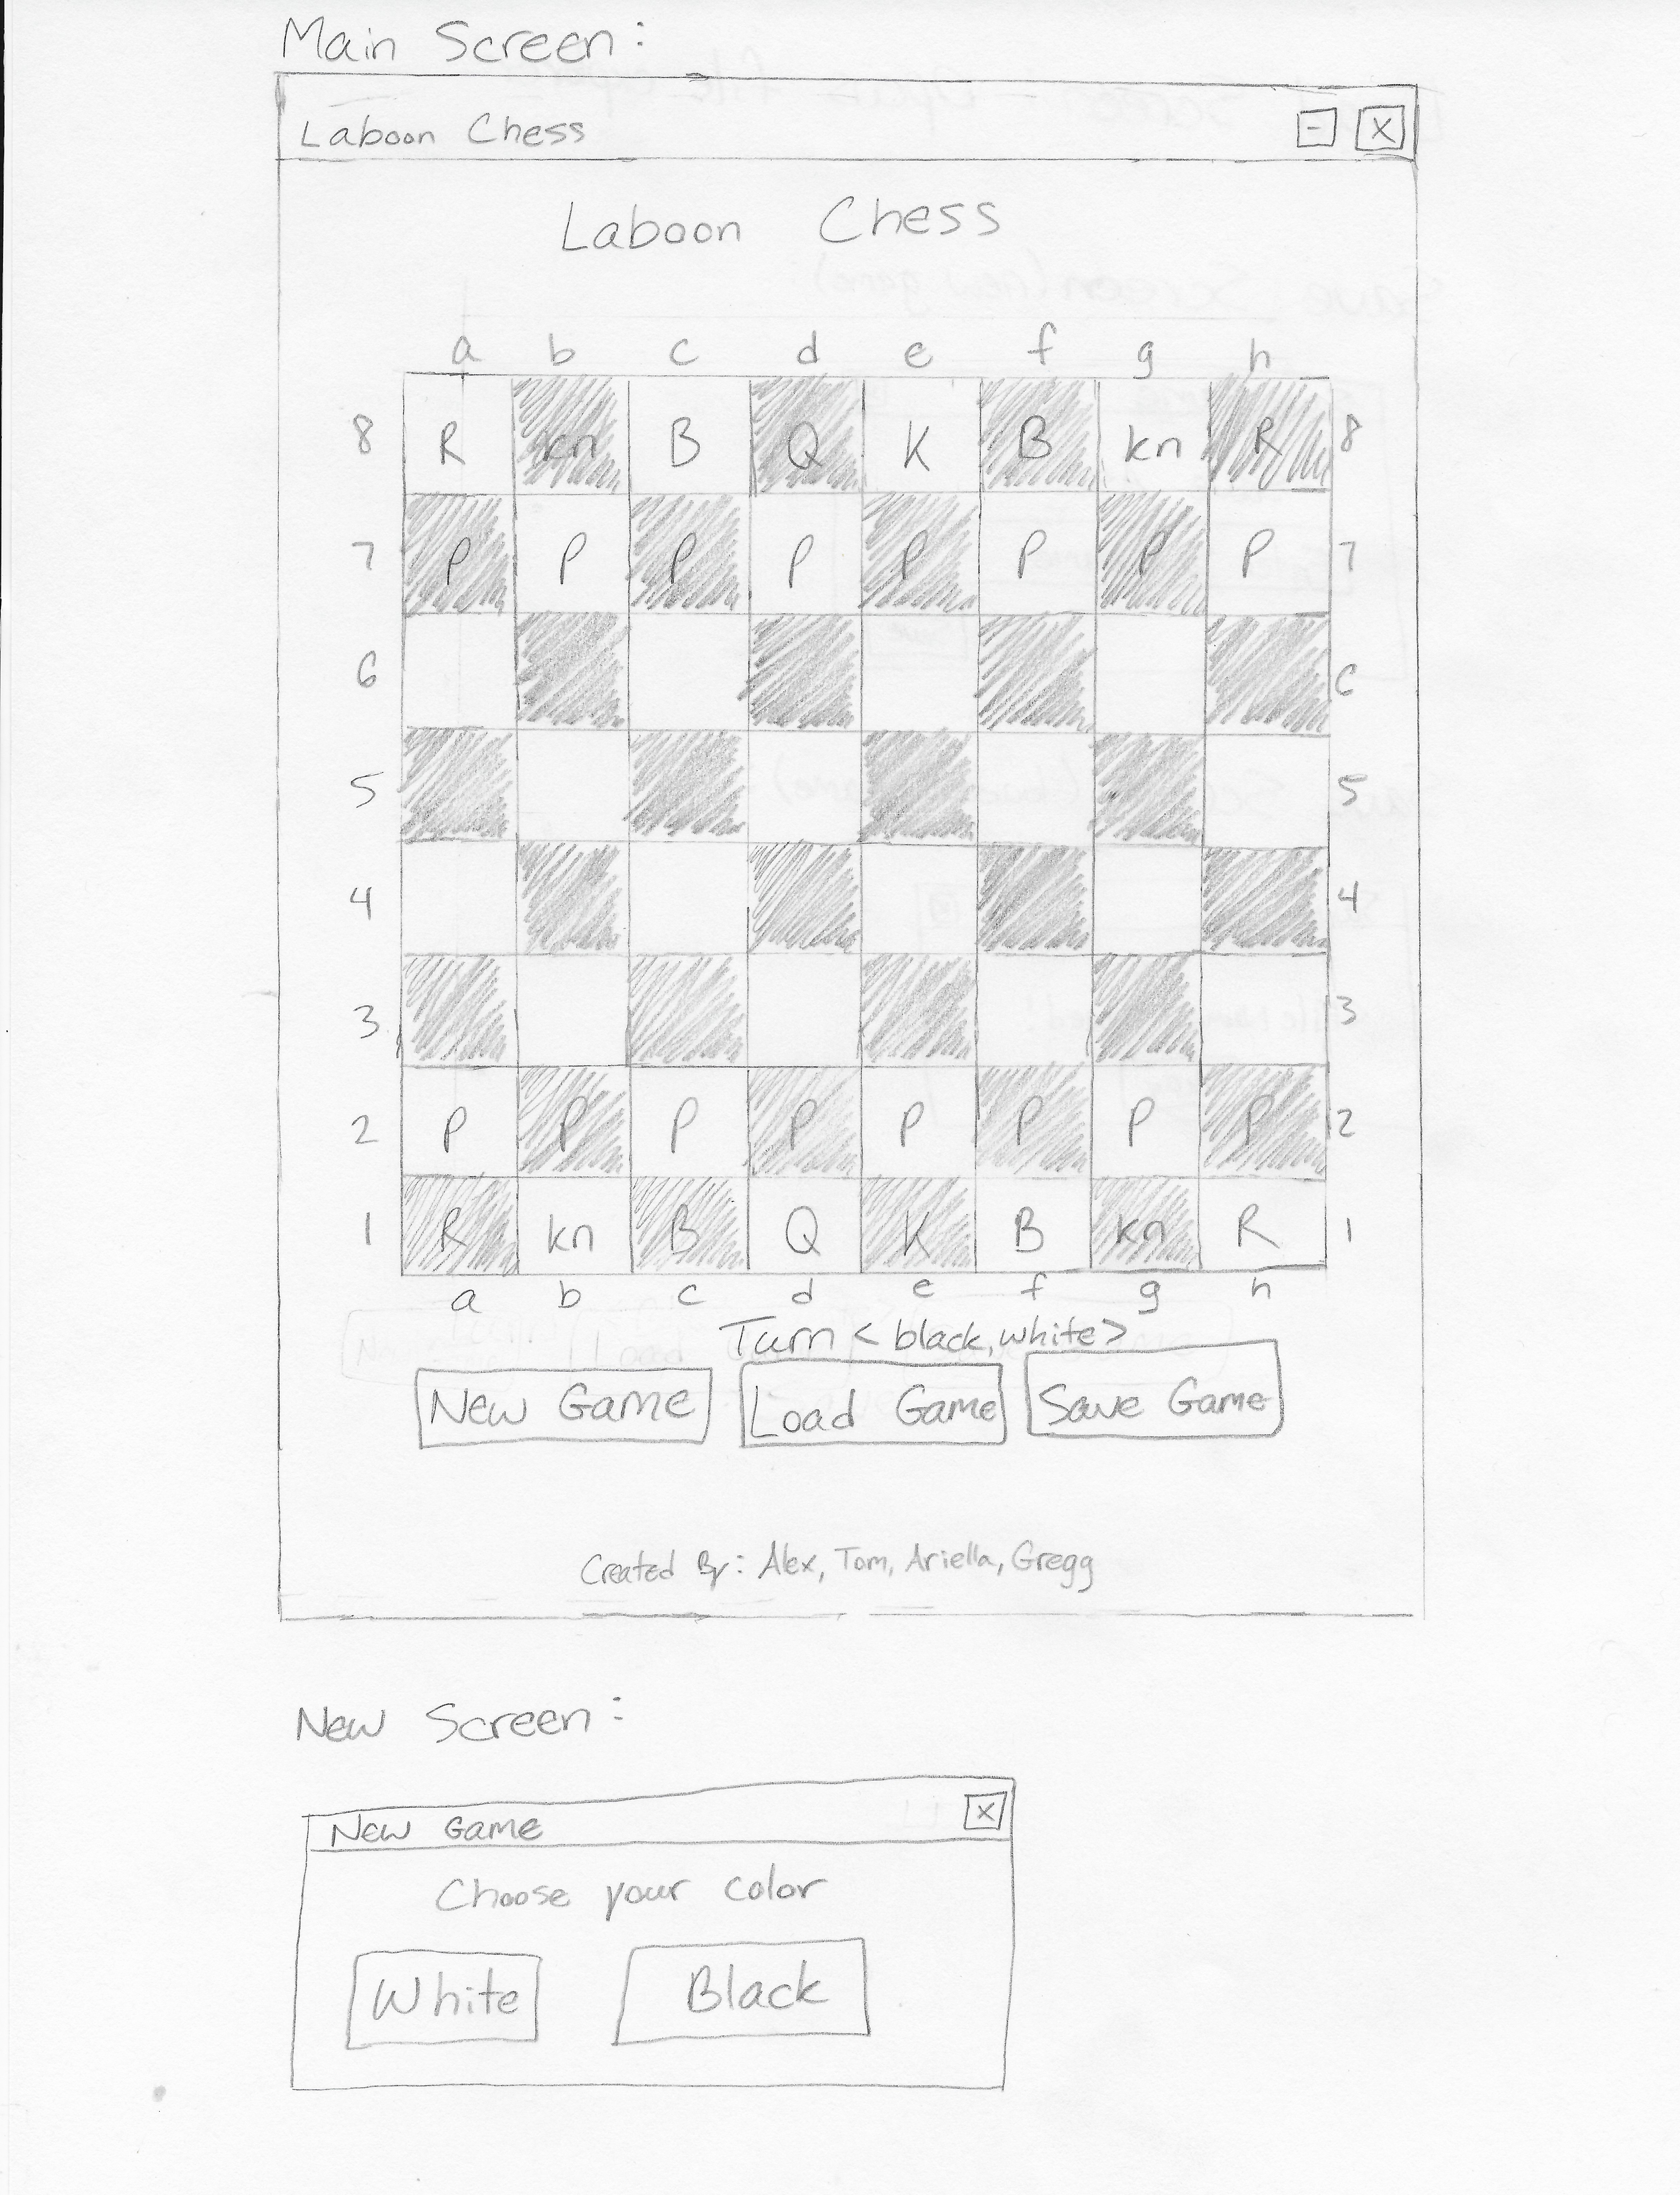
\includegraphics[width=\linewidth]{PaperProtoType.jpg}
		\label{fig:prototype1}
	\end{figure}
	\begin{figure}[H]
		\caption{Save screens}
		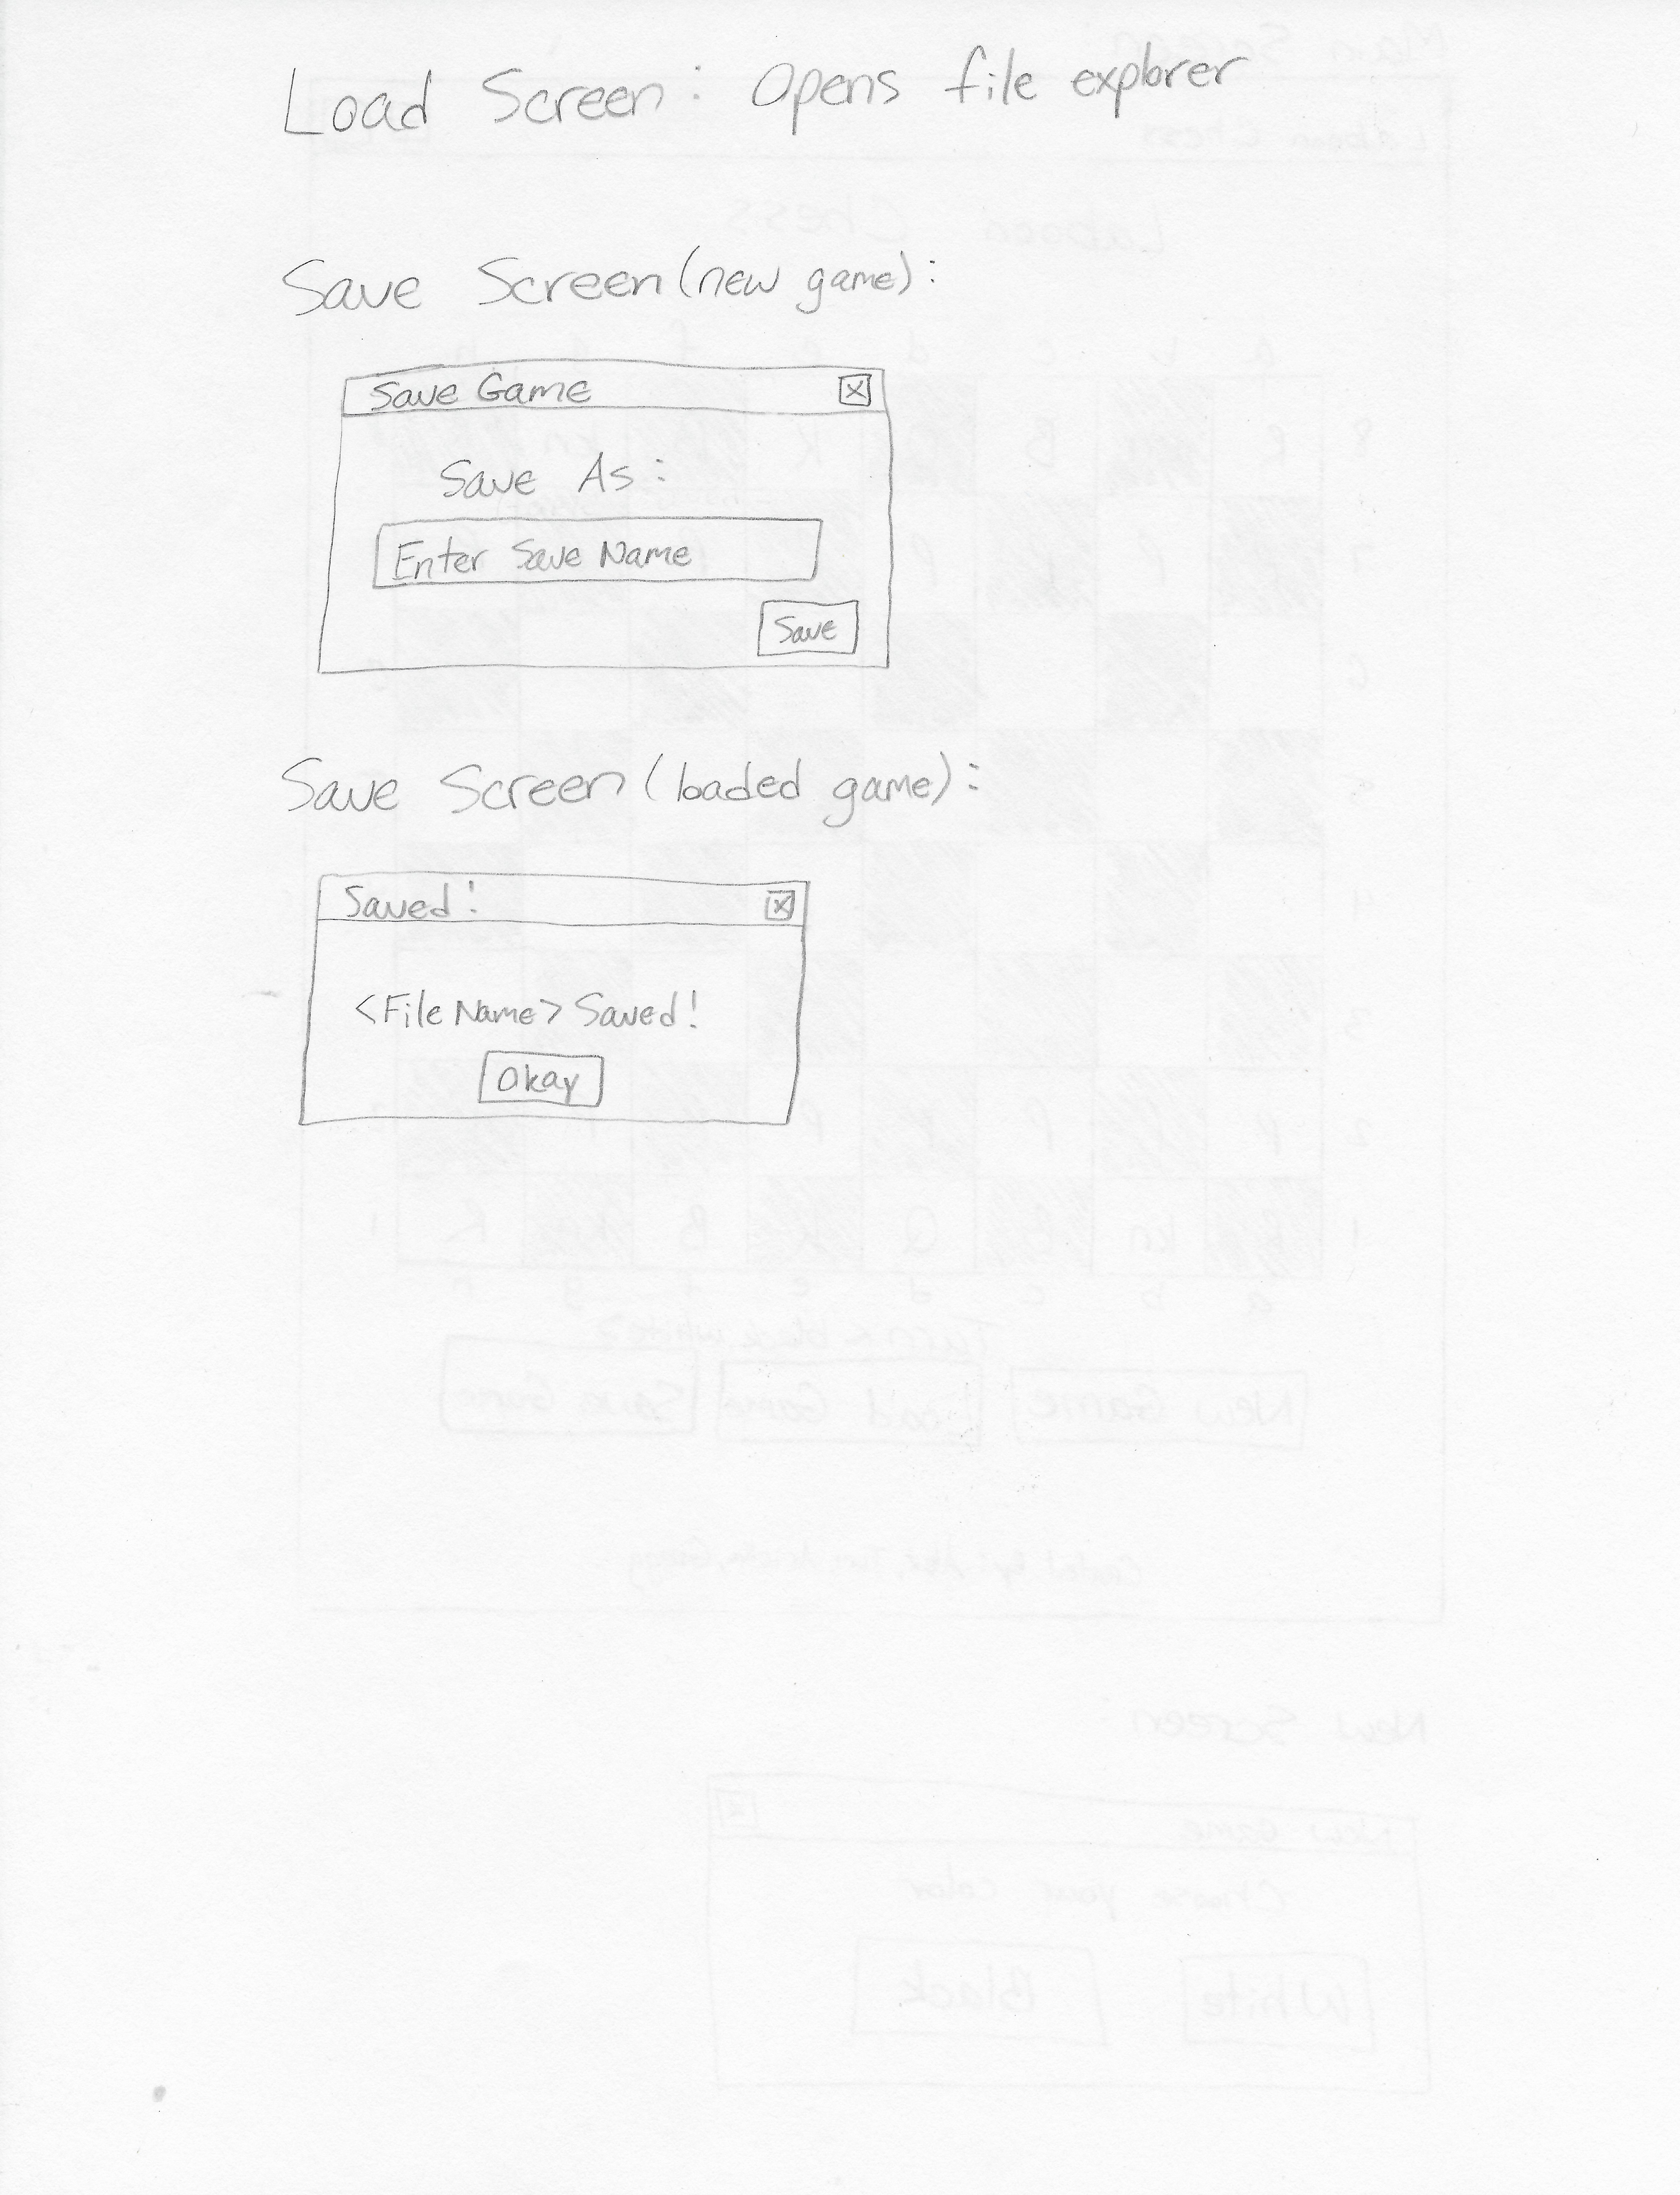
\includegraphics[width=\linewidth]{PaperProtoTypePart2.jpg}
		\label{fig:prototype2}
	\end{figure}
\end{document}